%
% File acl2018.tex
%
%% Based on the style files for ACL-2017, with some changes, which were, in turn,
%% Based on the style files for ACL-2015, with some improvements
%%  taken from the NAACL-2016 style
%% Based on the style files for ACL-2014, which were, in turn,
%% based on ACL-2013, ACL-2012, ACL-2011, ACL-2010, ACL-IJCNLP-2009,
%% EACL-2009, IJCNLP-2008...
%% Based on the style files for EACL 2006 by 
%%e.agirre@ehu.es or Sergi.Balari@uab.es
%% and that of ACL 08 by Joakim Nivre and Noah Smith

\documentclass[11pt,a4paper]{article}
\usepackage[hyperref]{acl2019}
\usepackage{times}
\usepackage{latexsym}
\usepackage{url}
\usepackage{graphicx}
\usepackage{booktabs}
\usepackage{bm}
\usepackage{amsfonts}
\usepackage{amsmath}
\usepackage{multirow}
\DeclareMathOperator*{\argmax}{arg\,max}
\DeclareMathOperator*{\argmin}{arg\,min}

\aclfinalcopy % Uncomment this line for the final submission
%\def\aclpaperid{***} %  Enter the acl Paper ID here

%\setlength\titlebox{5cm}
% You can expand the titlebox if you need extra space
% to show all the authors. Please do not make the titlebox
% smaller than 5cm (the original size); we will check this
% in the camera-ready version and ask you to change it back.

\newcommand\BibTeX{B{\sc ib}\TeX}

\newcommand{\dpcomment}[1]{\textcolor{green}{[#1 --deric]}}
\newcommand{\jbcomment}[1]{\textcolor{orange}{[#1 --josh]}}

\title{Syntactically Informed Natural Language Inference}

\author{
  Deric Pang \quad
  Joshua Bean \\
  Paul G. Allen School of Computer Science \& Engineering \\
  University of Washington \\
  Seattle, WA, USA \\
  {\tt \{dericp, jbean96\}@cs.washington.edu} \\
}

\date{}

\begin{document}
\maketitle
\begin{abstract}
We demonstrate the importance of syntactic information in semantic models by extending the
decomposable attention model \citep{Parikh2016-em} for natural language inference
to use syntactic features.
By pipelining the hidden states of a neural syntax parser into the decomposable
attention model, we achieve greater performance on the SciTail dataset
\citep{Khot2018-th} than what is gained by
using contextual embeddings like ELMo \citep{Peters2018-fz}.
\end{abstract}

\section{Introduction}

Natural language inference (NLI) is the task of characterizing entailment and
contradiction relationships between texts. We improve NLI models by adding syntactic
features into existing models.

In general, most NLI tasks are formulated as characterizing the relationship
between a pair of sequences---a premise and a hypothesis. An NLI model should
predict whether the hypothesis is entailed by the premise, contradicts the
premise, or is neutral to the premise.

We extend the decomposable attention (DA) model by \citet{Parikh2016-em}
incorporating syntactic features.
\dpcomment{Include brief summary of contributions here.}
The DA model obtained state-of-the-art results on the
SNLI \citep{Bowman2015-is} dataset at its time of publication while using
drastically fewer parameters than previous NLI models.
We primarily
evaluate on the domain specific Scitail dataset \citep{Khot2018-th}
for both its smaller size and lack of annotation artifacts when compared to SNLI
\citep{Gururangan2018-lj}.

Our model, \textbf{syntail}, achieves \dpcomment{add number here} better 
test accuracy than the vanilla
DA model and \dpcomment{add number here} better test accuracy than DA with ELMo all
while maintaining the core DA architecture.

\section{Decomposable Attention Model}

The DA model is a simple and easily parallelizable approach to NLI.
We summarize it here so we can build upon it later.
The model
decomposes into attend, compare, and aggregate steps.

Let
$\bm{p} = \langle p_1, \dots, p_{\ell_p} \rangle$ and
$\bm{h} = \langle h_1, \dots, h_{\ell_h} \rangle$ where each $p_i, h_i \in \mathbb{R}^d$
is a $d$ dimensional word embedding vector.

\paragraph{Attend.} Compute unnormalized attention weights $e_{ij}$ with
a feed-forward neural network $F$:
\begin{align}\label{eq:attend}
    e_{ij} := F(p_i)^\mathsf{T} F(h_j).
\end{align}
Compute the aligned subphrases $\bm{H}i$ and $\bm{P}_j$:
\begin{align}
    \bm{H}_i &:= \sum_{j=1}^{\ell_h}\frac{\exp{(e_{ij})}}
                                        {\sum_{k=1}^{\ell_h}\exp{(e_{ik})}}h_j\,, \notag \\
    \bm{P}_j &:= \sum_{i=1}^{\ell_p}\frac{\exp{(e_{ij})}}
                                        {\sum_{k=1}^{\ell_h}\exp{(e_{ik})}}p_i\
\end{align}
where $\bm{H}_i$ is the weighted sum over $\bm{h}$ that aligns to $p_i$ and vice versa
for $\bm{P}_j$.

\paragraph{Compare.} Compare each $(p_i, \bm{H}_i)$ and $(h_j, \bm{P_}j)$ pairs
with another feed-forward neural network $G$:
\begin{align}
    \bm{v}^p_i &:= G([p_i, \bm{H}_i])\quad \forall i \in [1,\ldots, \ell_p]\,, \notag \\
    \bm{v}^h_j &:= G([h_j, \bm{P}_j])\quad \forall j \in [1,\ldots, \ell_h]\,.
\end{align}

\paragraph{Aggregate.} Aggregate each set of comparison vectors:
\begin{align}
\bm{v}^p = \sum_{i=1}^{\ell_p} \bm{v}^p_i \qquad\,, \qquad
\bm{v}^h = \sum_{j=1}^{\ell_h}  \bm{v}^h_j\,.
\end{align}
and make a prediction with a final feed-forward layer $H$:
\begin{align}\label{eq:predict}
    \hat{\bm{y}} = H([\bm{v}^p, \bm{v}^h]).
\end{align}

\section{Our Model}

The motivation for incorporating syntactic information in an NLI model
can be demonstrated with a simple example. Consider the premise ``Adrian is running
and Alex is swimming." If we present the DA model trained on SNLI with the
hypothesis ``Adrian is swimming," it will confidently predict that this
blatantly incorrect hypothesis is entailed by the premise. Observing
any syntactic parse of
the premise will make it obvious that Adrian is in fact running.

Incorporating syntactic information in semantic tasks has been investigated
before by \dpcomment{add references and discussion}.

Our model, \textbf{syntail}, extends the DA model.
We experiment with features generated by two syntax parsers---the
minimal span-based neural constituency parser \citep{Stern2017-co} and
the deep biaffine attention model for dependency parsing \citep{Dozat2016-gs}. We also experiment
with different methods of incorporating the syntactic features extracted
from these parsers.

\subsection{Extracting Syntactic Information}

The minimal span-based neural constituency parser and the deep biaffine attention
model for dependency parsing both encode the input sequence with an LSTM. Using
this LSTM, we obtain
syntactic features $\bm{s}^p = \langle s^p_1, \dots, s^p_{\ell_p} \rangle$ and
$\bm{s}^h = \langle s^h_1, \dots, s^h_{\ell_h} \rangle$ from the premise and hypothesis,
respectively. An $s_i$ is either
the final hidden state $\bm{r}_i$ of the LSTM at index $i$ or a projected
representation of $\bm{r}_i$.

\subsection{Syntail Architectures}

We will now describe the different model architectures we experimented with.
In general, as the version number increases, the complexity of the model increases.

\paragraph{v1: Naive late fusion of syntactic features.}
The simplest way to incorporate $\bm{s}$ is to concatenate its final representation to
$\bm{v}^p$ and $\bm{v}^h$ as shown in figure~\ref{fig:v1}.

\begin{figure}[h]
    \centering
    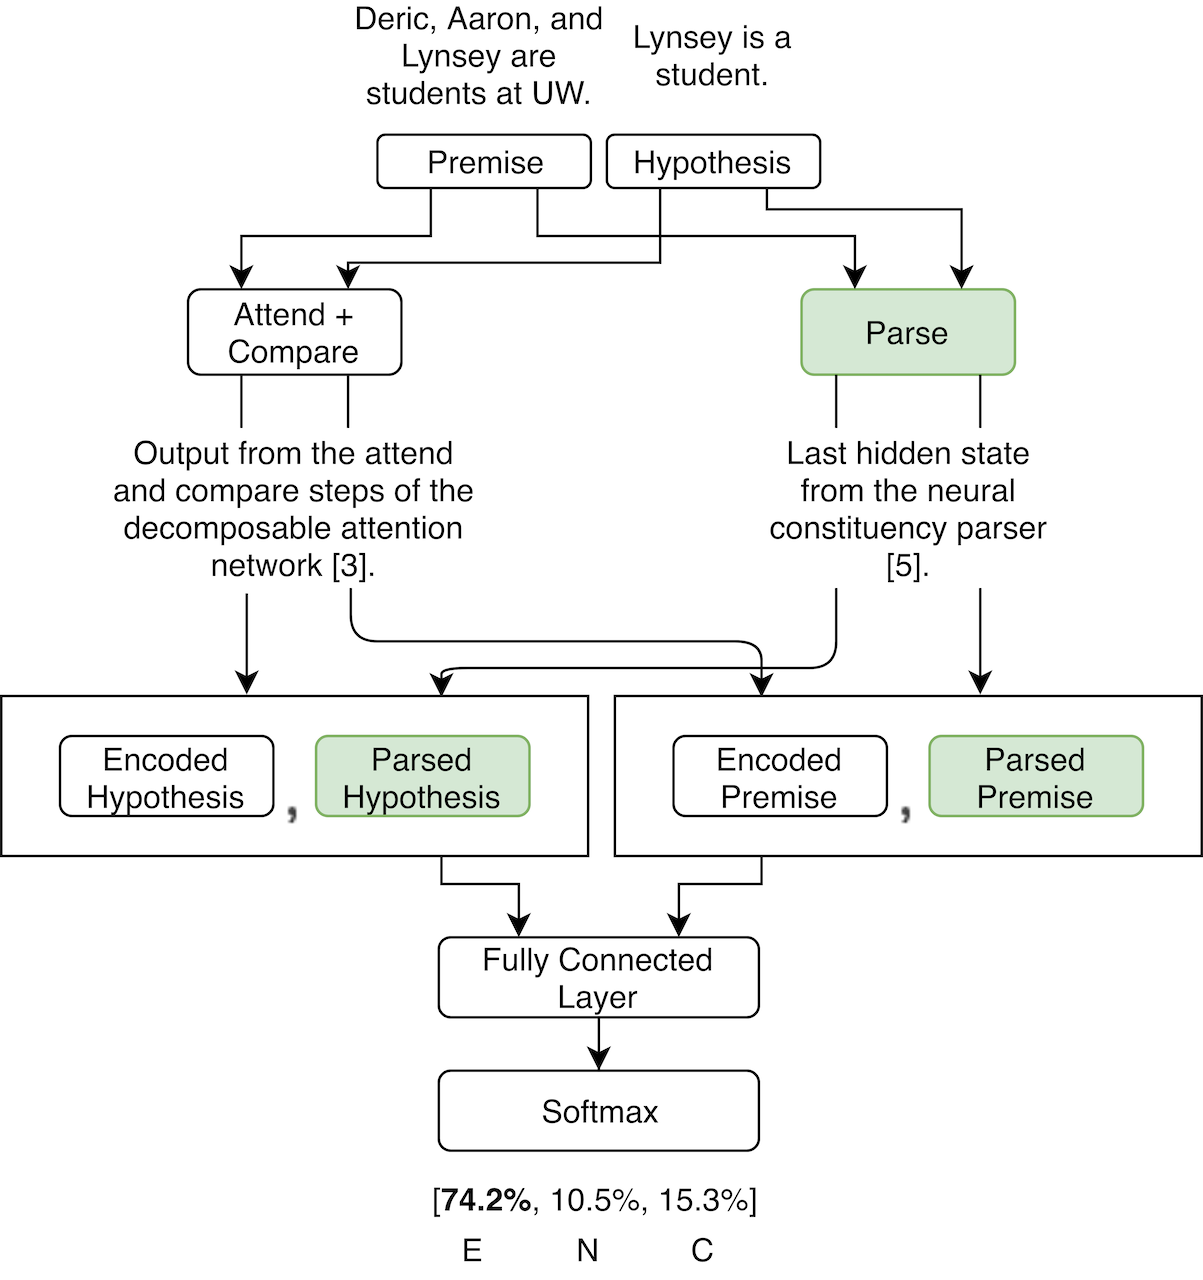
\includegraphics[width=\linewidth]{figures/v1.png}
    \caption{Syntail v1 architecture.}
\label{fig:v1}
\end{figure}

The prediction step in equation~\ref{eq:predict} then becomes:
\begin{align}
    \hat{\bm{y}} = H([\bm{v}^p, s^p_{\ell_p}, \bm{v}^h, s^h_{\ell_h}])
\end{align}
where we concatenate the final hidden representation of the premise and hypothesis
when passed through the neural syntax parser with the aggregrated comparision vectors.
Everything else is identical to the DA model.

\paragraph{v2: Using syntactic features to attend.}
We wanted to experiment with incorporating syntactic features earlier in the model.
Instead of learning weights on the syntactic features, it is possible to
concatenate them to the projected input representations as show in figure~\ref{fig:v2}.

\begin{figure}[h]
    \centering
    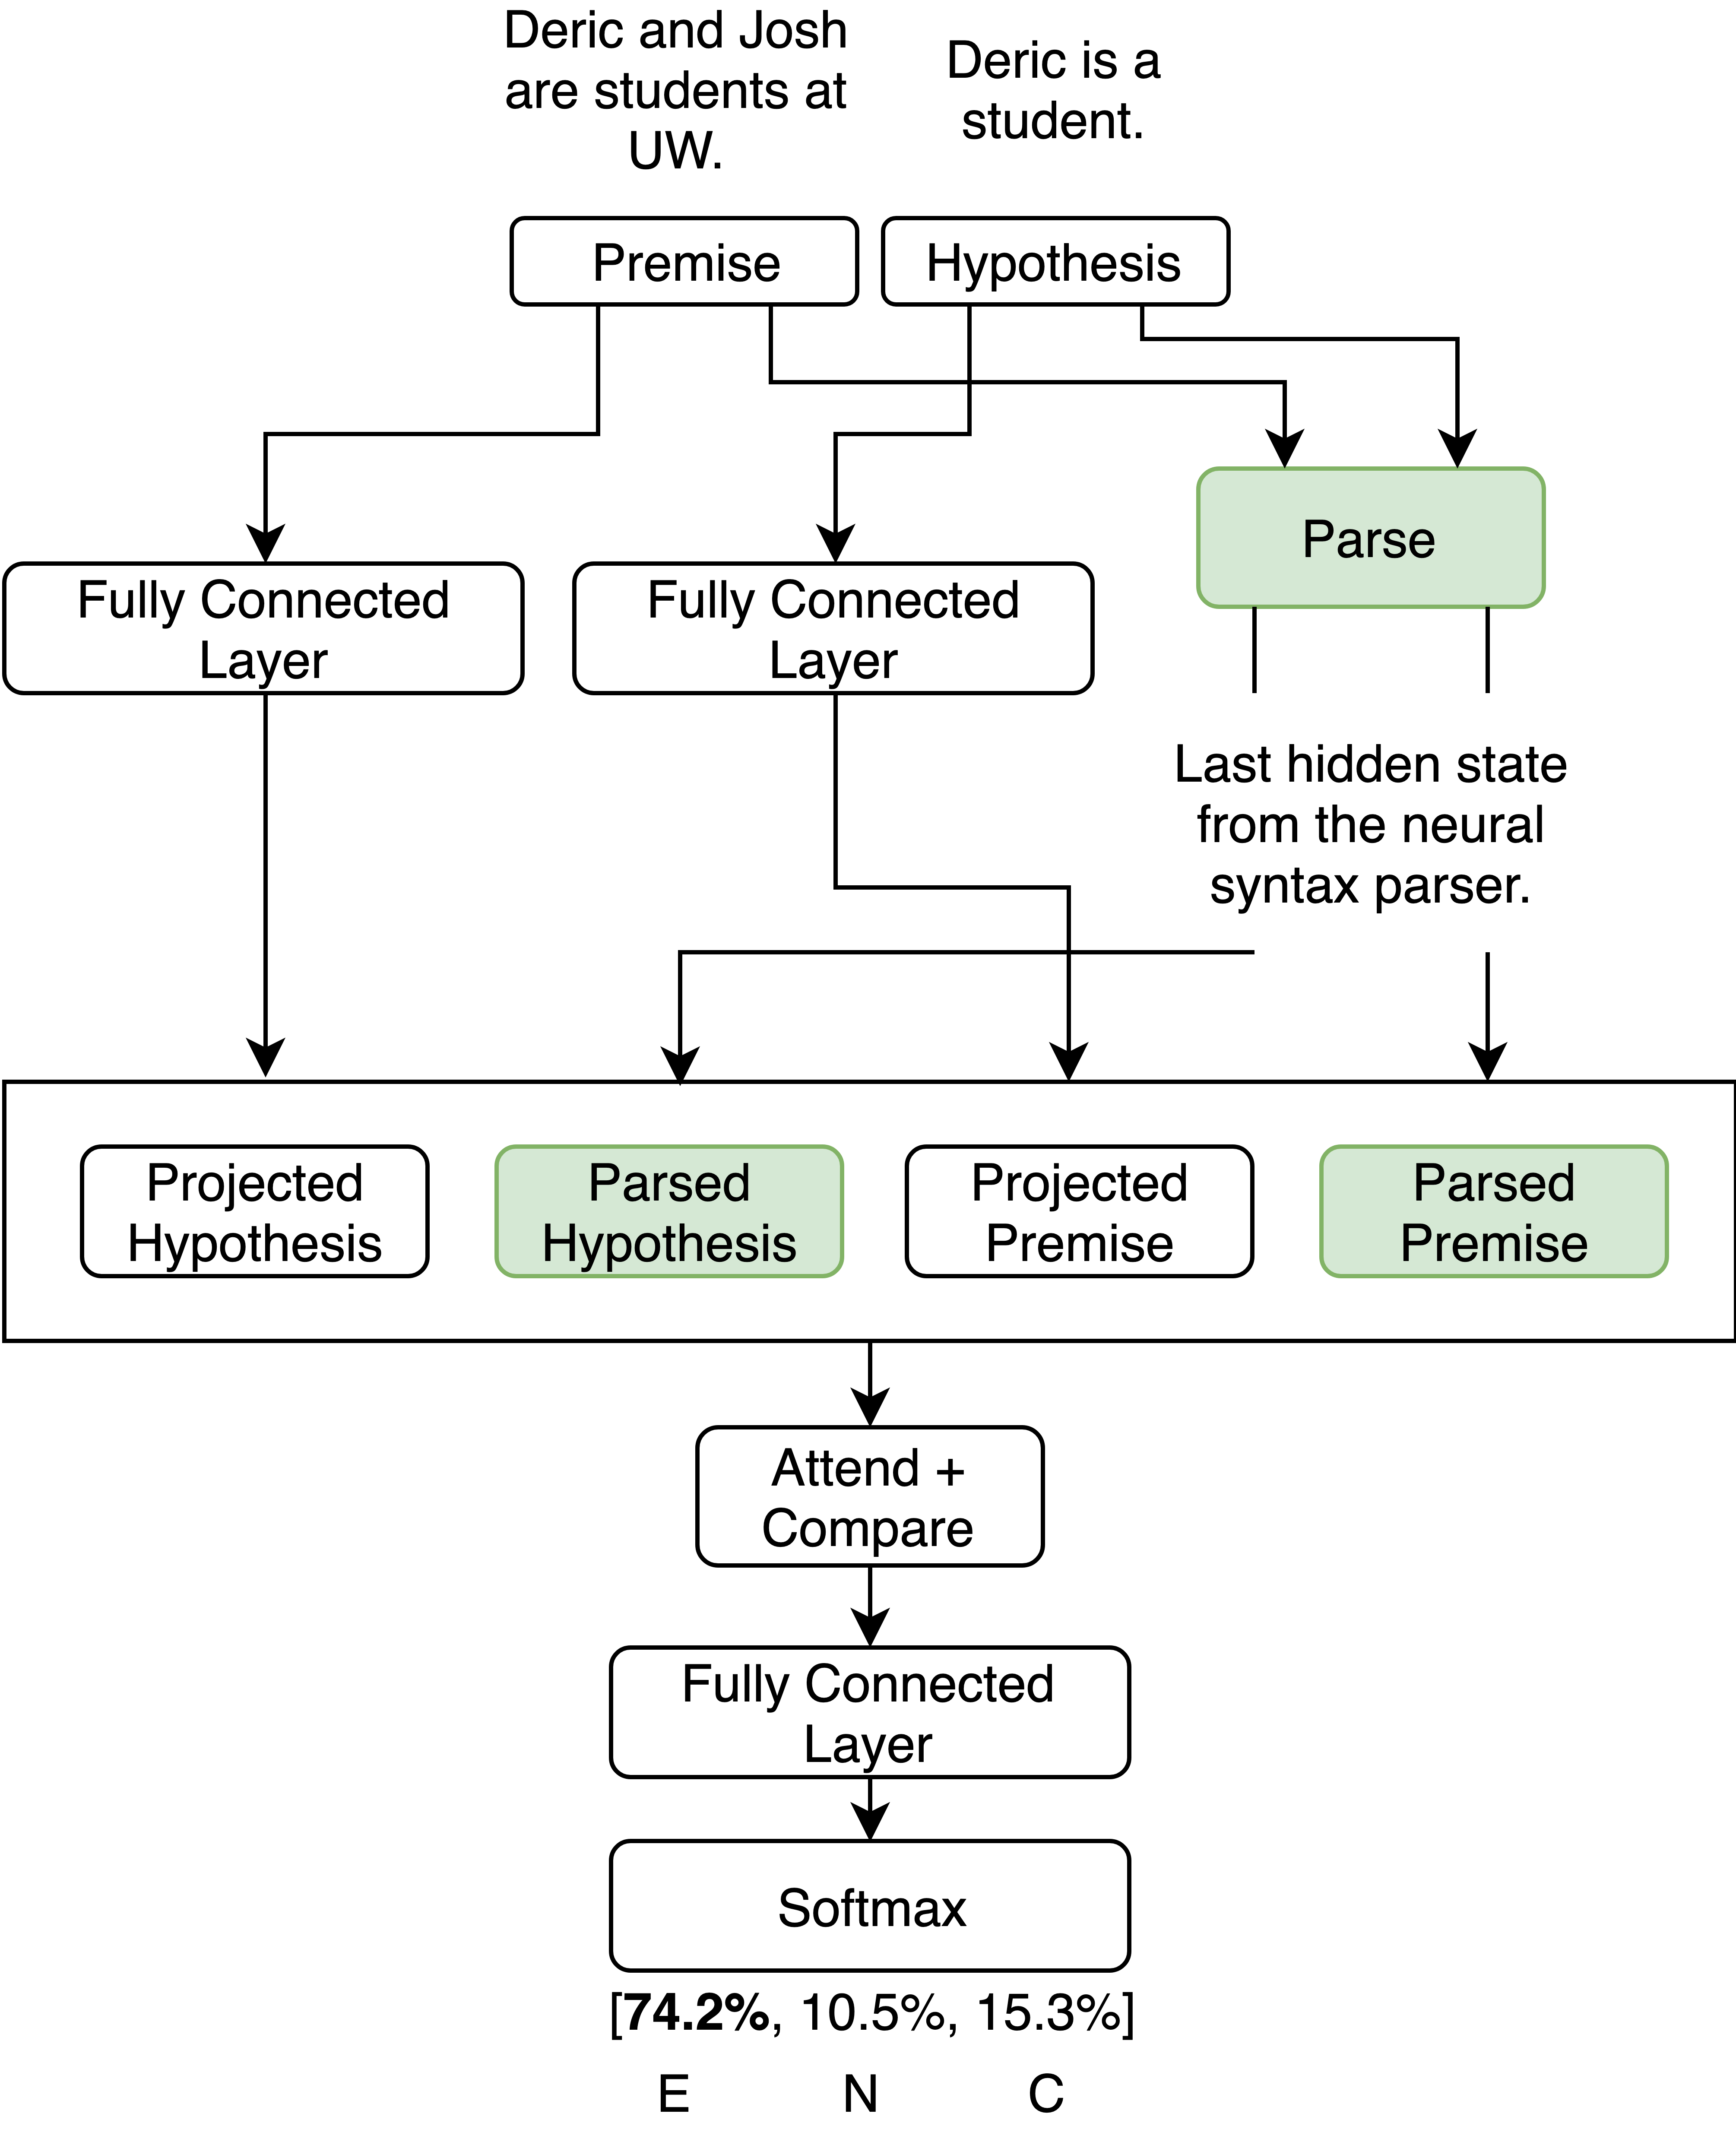
\includegraphics[width=\linewidth]{figures/v2.png}
    \caption{Syntail v2 architecture.}
\label{fig:v2}
\end{figure}

Computing the
unnormalized attention weights in equation~\ref{eq:attend} then becomes:
\begin{align}
    e_{ij} := [F(p_i), s^p_i]^\mathsf{T} [F(h_j), s^h_i]
\end{align}
where instead of calculating the alignment using only the 
projected hypothesis and premise vectors, we now also use final hidden states of
the premise and hypothesis when passed through the neural syntax parser.
This seems rather naive since this model will not
learn any weights on the syntactic features, but in practice this model
performs very well. Everything else is identical to the DA model.

\paragraph{v3: Using syntactic features to project the premise and hypothesis.}
We decided to try incorporating the syntactic features even earlier in the model.
Instead of concatenating the final hidden states of the parsed premise and hypothesis
with the projected inputs, we concatenate the final hidden states of the parsed
premise and hypothesis with in the inputs immediately before projecting them. This
architecture is shown in figure~\ref{fig:v3}.

\begin{figure}[h]
    \centering
    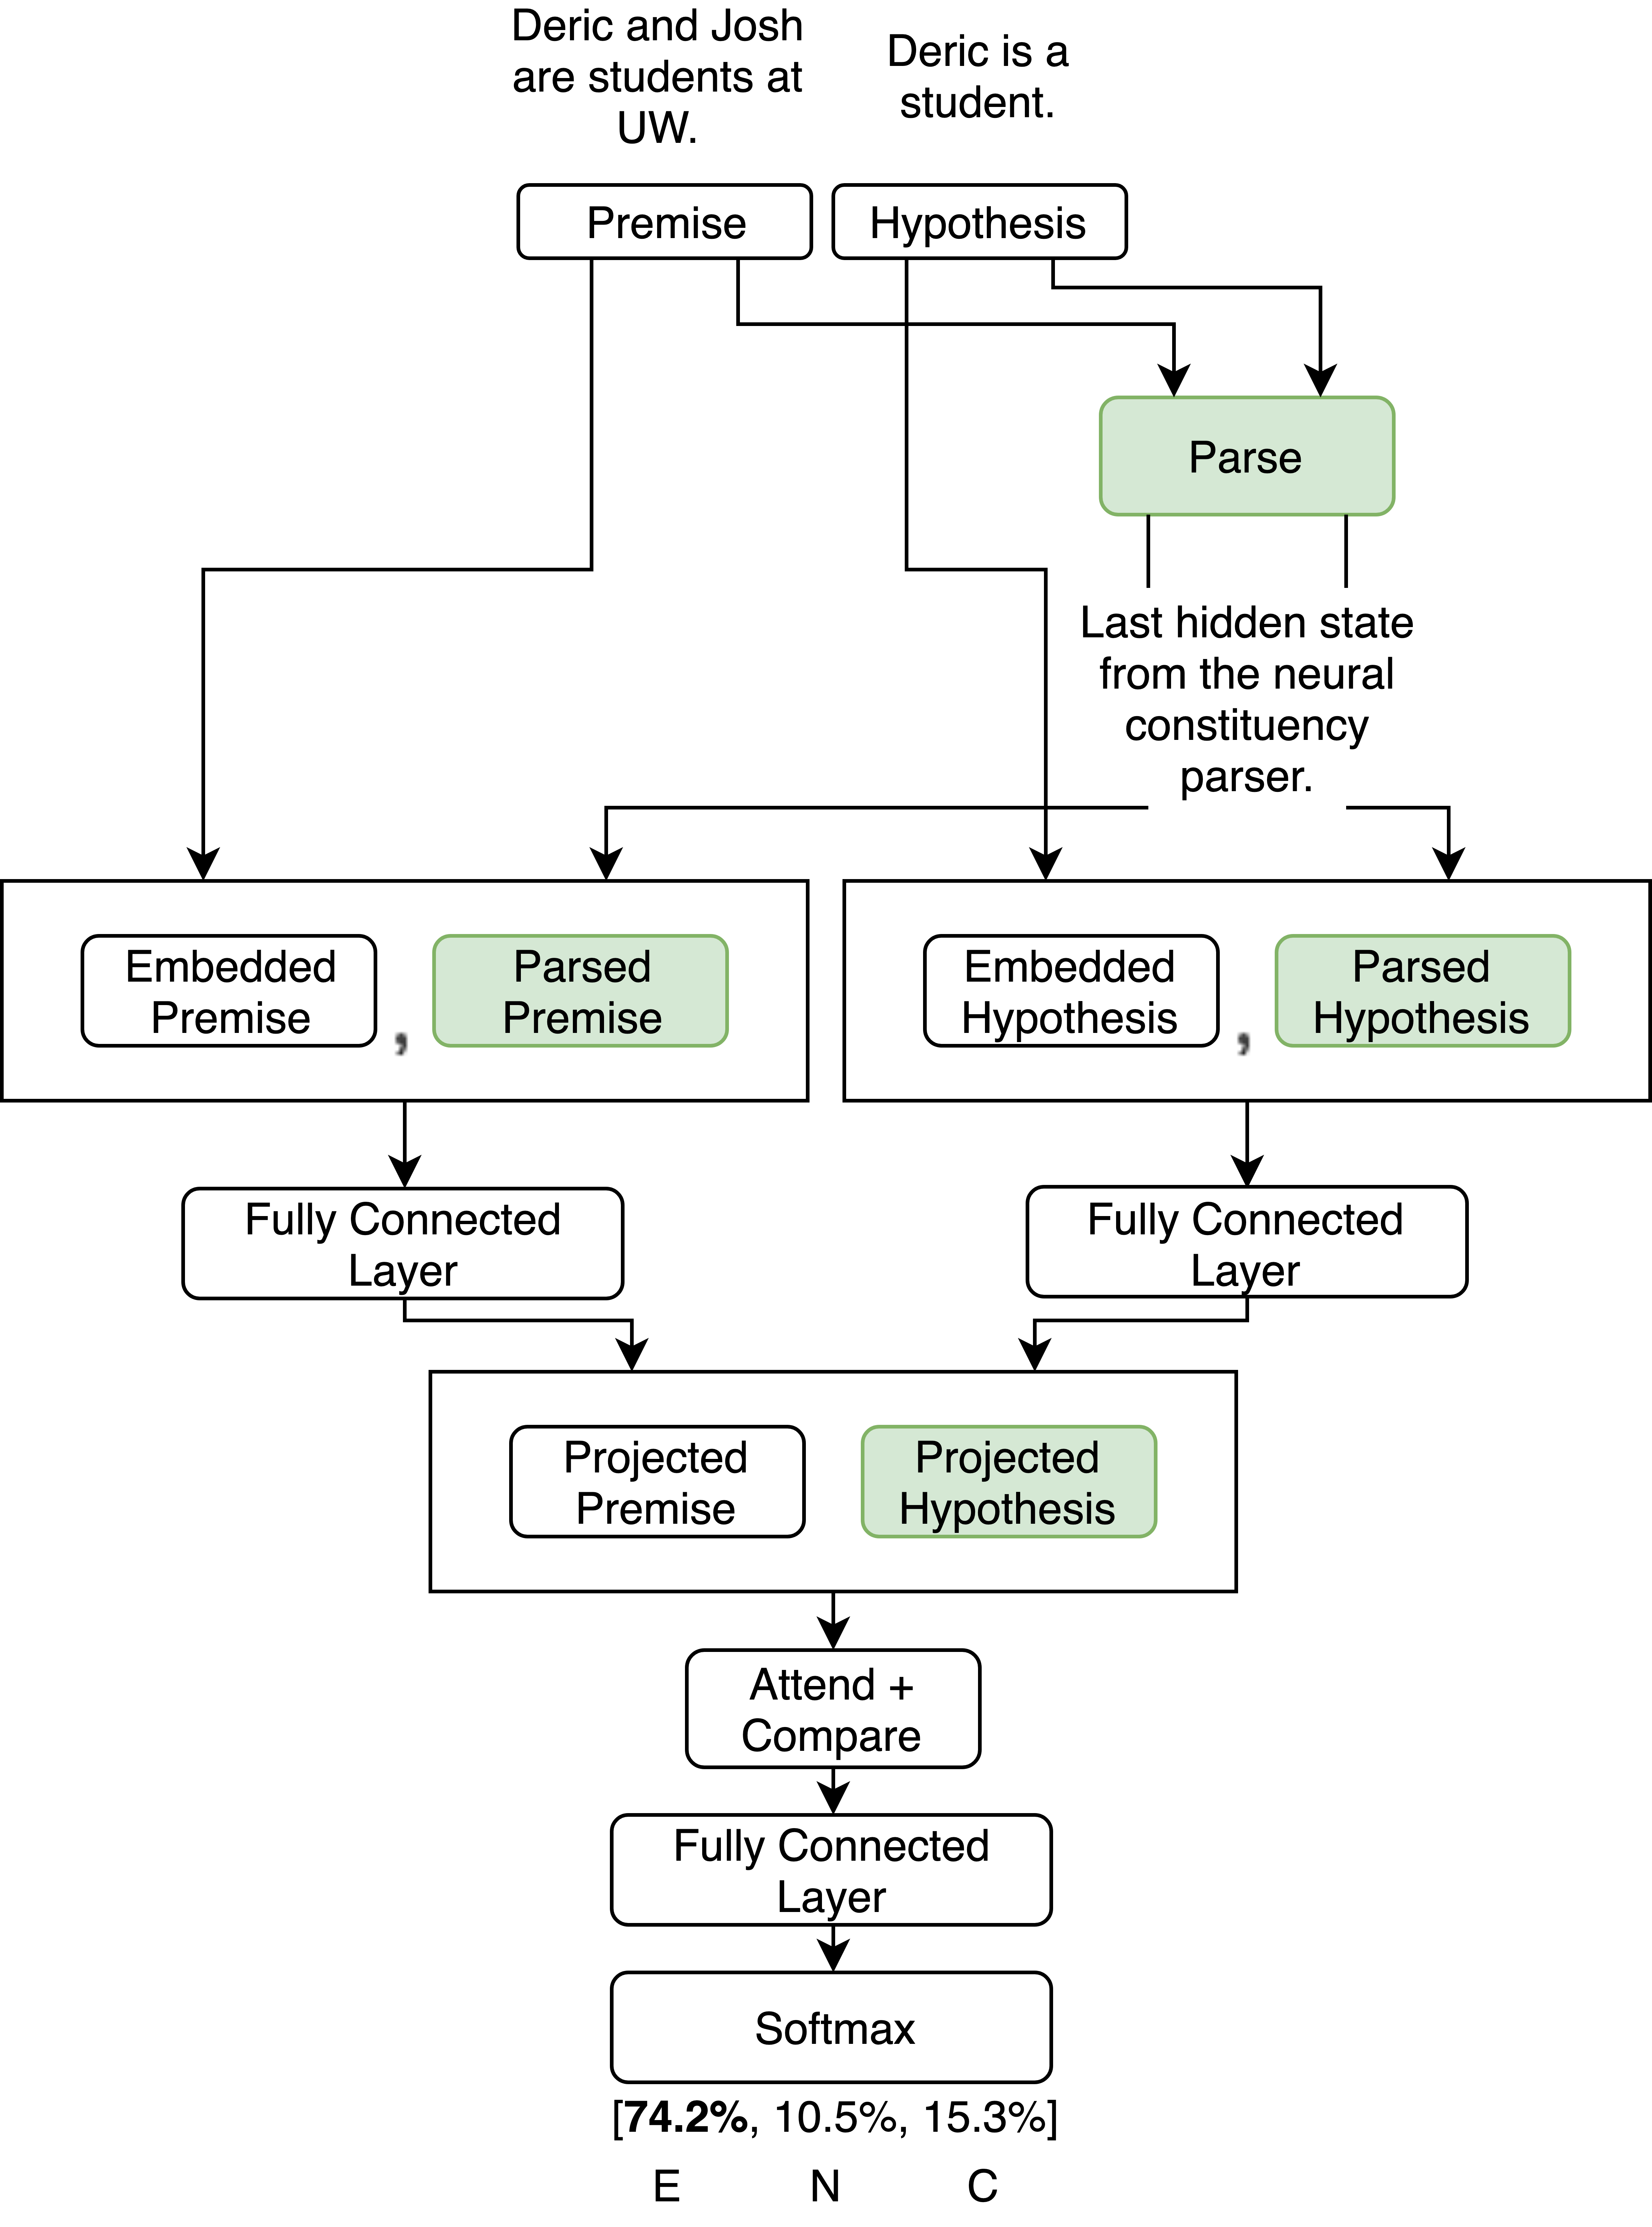
\includegraphics[width=\linewidth]{figures/v3.png}
    \caption{Syntail v3 architecture.}
\label{fig:v3}
\end{figure}

Computing the unnormalized attention weights in equation~\ref{eq:attend} then becomes:
\begin{align}
    e_{ij} := F([p_i, s^p_i])^\mathsf{T} F([h_j, s^h_j]).
\end{align}
Everything else is identical to the DA model.

\paragraph{v4: Projecting the syntactic features before computing attention.}
After noticing a drop in performance from v2 to v3, we hypothesized that it was
due to not allowing our model to transform the syntactic features enough before
calculating attention.
We decided to learn weights to project the final hidden states of the parsed
premise and hypothesis by passing them through an additional fully-connected layer before 
concatenating them to the inputs. This architecture is shown in figure~\ref{fig:v4}

\begin{figure}[h]
    \centering
    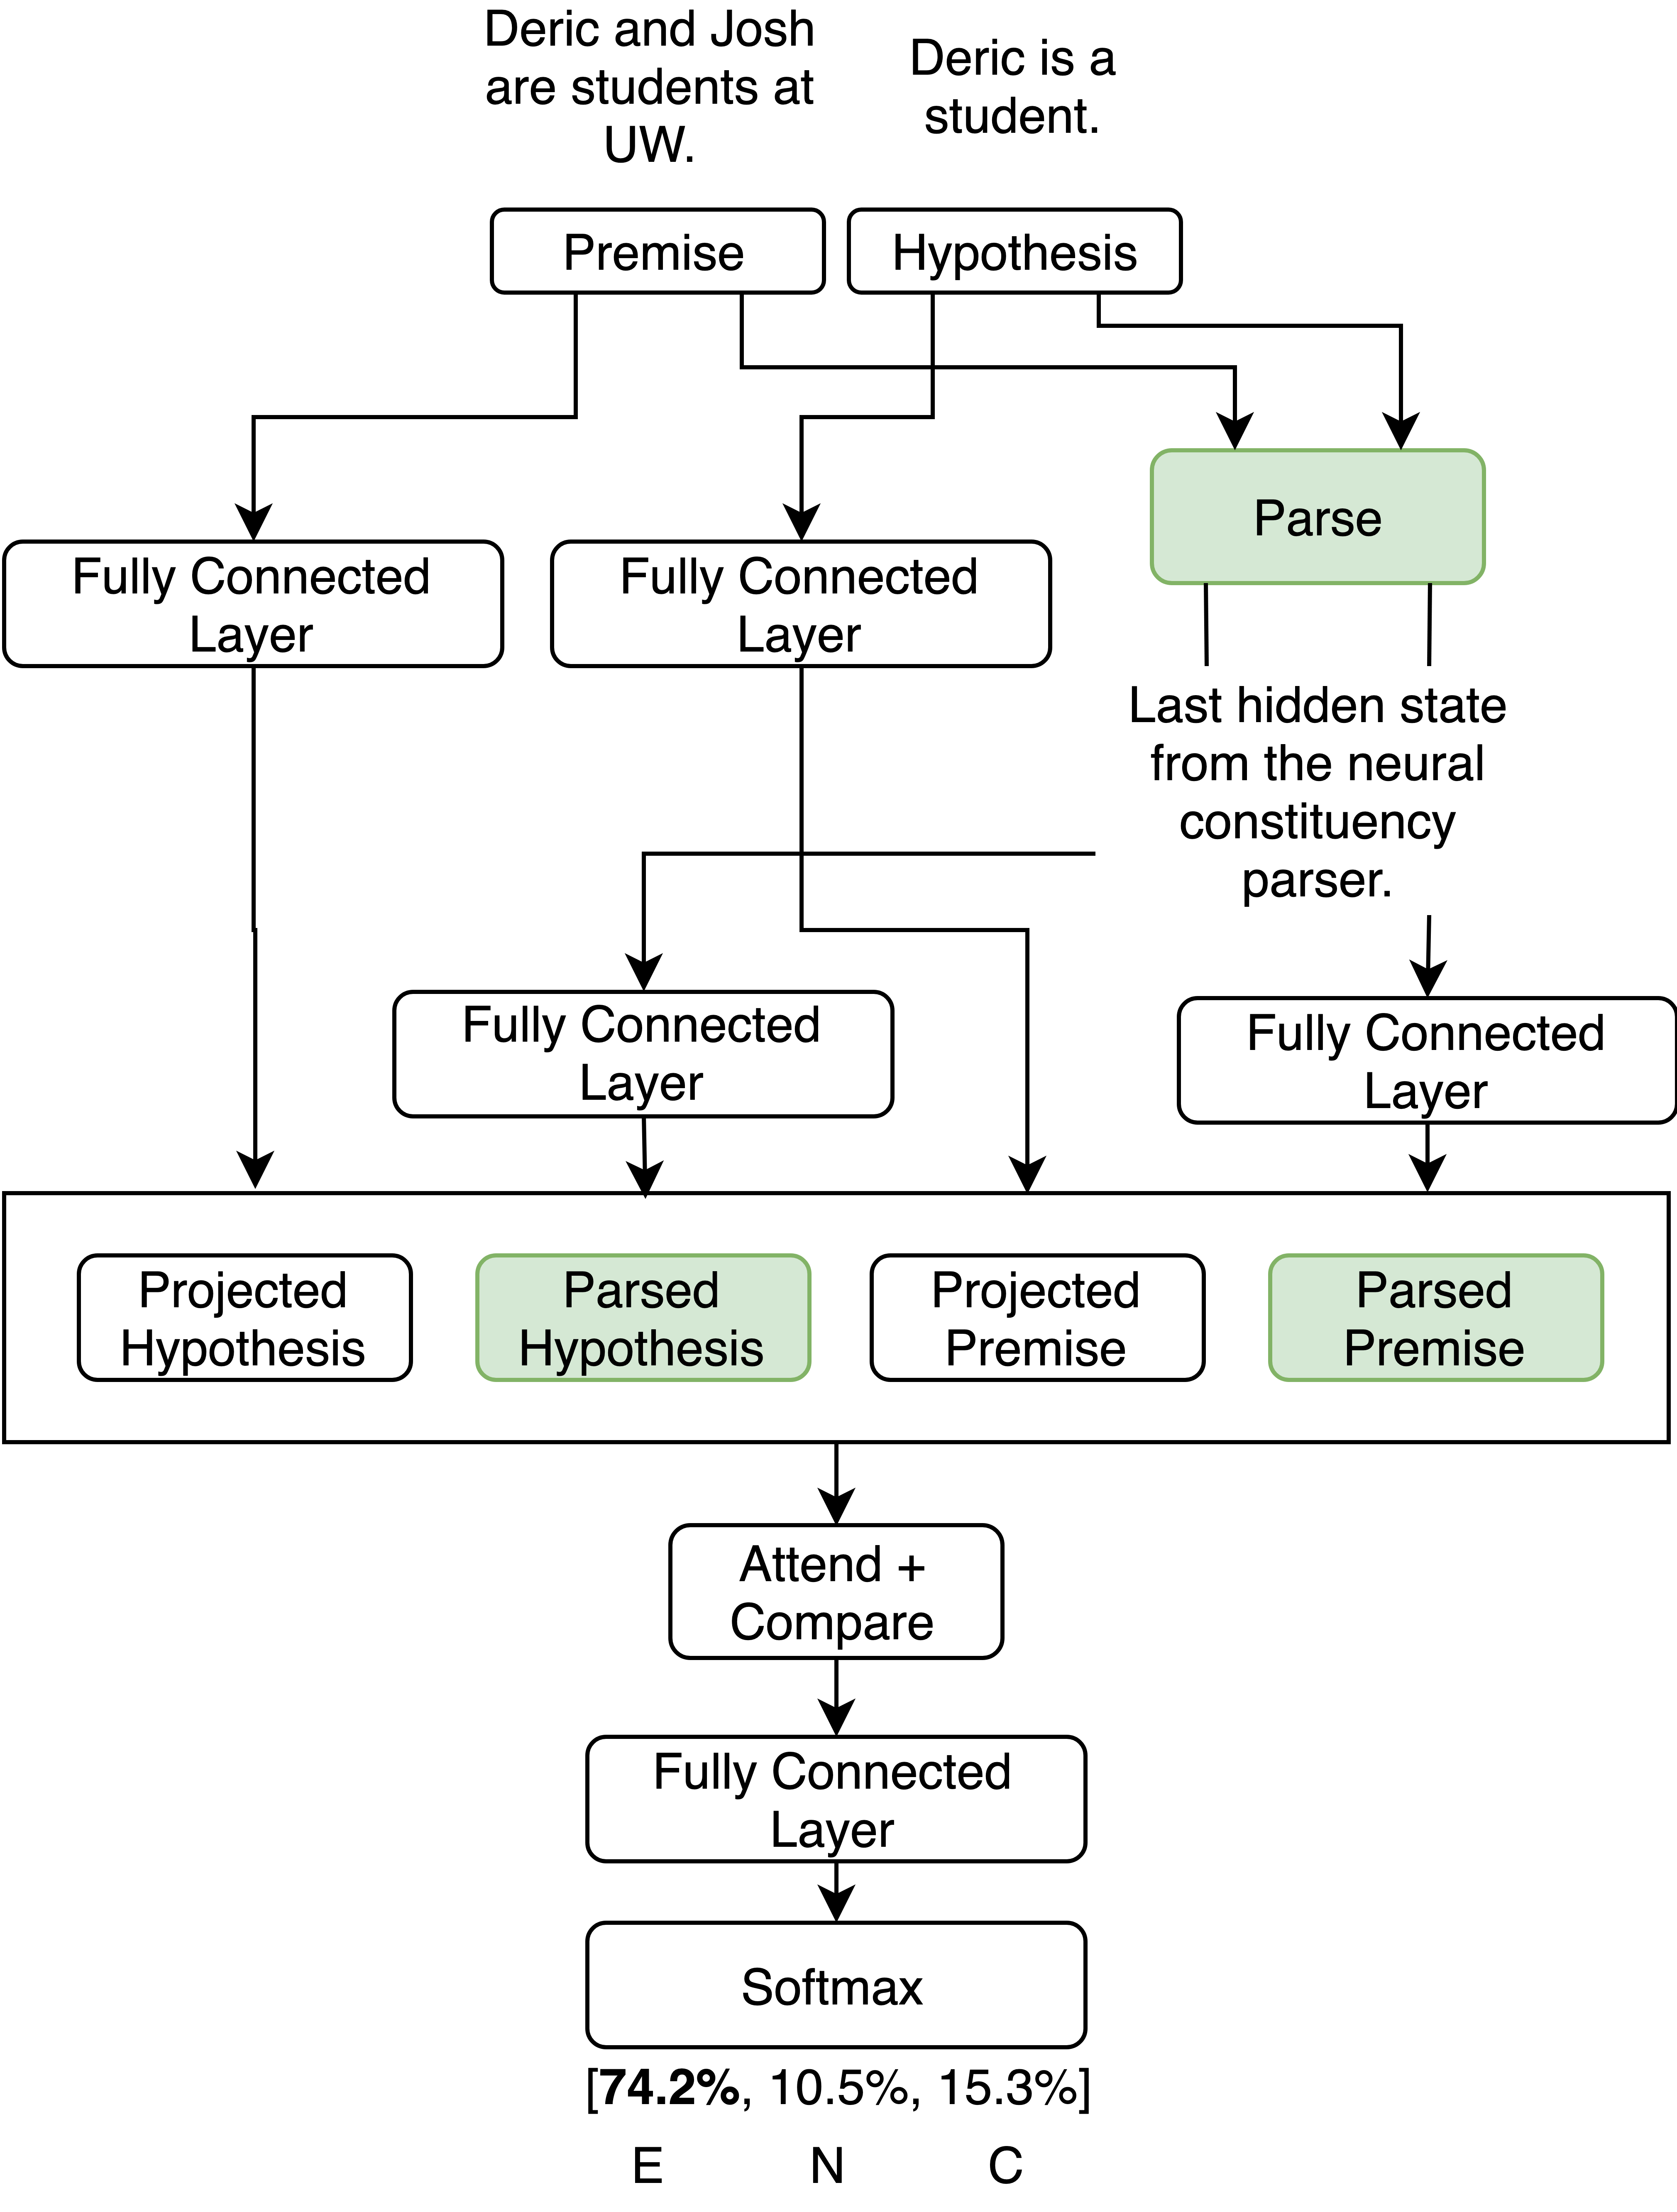
\includegraphics[width=\linewidth]{figures/v4.png}
    \caption{Syntail v4 architecture.}
\label{fig:v4}
\end{figure}

Computing the unnormalized attention weights in equation~\ref{eq:attend} then becomes:
\begin{align}
    e_{ij} := F([p_i, J(s^p_i)])^\mathsf{T} F([h_j, J(s^h_j)])
\end{align}
where $J$ is a feed-forward neural network.
Everything else is identical to the DA model.

% \jbcomment{If we're only using data from the dependency parser we should probably 
% remove the section following this comment}
% Supplemental variations were done on top of these restructures of the network. One 
% of the variations that we introduced was a retrained constituency parser. By 
% retraining the constituency parser on the Penn Treebank dataset \citep{marcus1993building} 
% we could change the dimensions of the encoded syntax vectors to better fit with our models. 
% Additionally, we experimented with training our models using the dependency parser model 
% derived by \citet{Dozat2016-gs} to see if the different types of encoded parses influenced 
% the performance of the network.

\subsection{Implementation Details}
\dpcomment{Add some hyper-parameter stuff here.}

\section{Experiments}

We compare our model's performance to the decomposable attention model
\citep{Parikh2016-em} and the ESIM model \citep{Chen2016-wl}.

\begin{table}[h]
\centering
\resizebox{\linewidth}{!}{
\begin{tabular}{cccccc} 
\toprule
Model          & Embeddings      & Dev. Acc. & Test Acc.  \\ 
\midrule
Majority Class & n/a             & 63.3      & 60.3       \\
N-Gram         & n/a             & 65.0      & 70.6       \\
ESIM           & GloVe 840B 300d & 70.5      & 70.6       \\
DA             & GloVe 6B 300d   & 70.4      & 72.6       \\
DA             & ELMo            & 79.1      & 75.5       \\
\midrule
Syntail v2     & GloVe 6B 300d   & 79.3      & ?          \\
Syntail v3     & GloVe 6B 300d   & 82.3      & 77.4       \\
Syntail v5     & GloVe 6B 300d   & ?         & ?          \\
Syntail v7     & GloVe 6B 300d   & 81.3      & 77.0       \\
\bottomrule
\end{tabular}}
\label{table:experiments}
\caption{\dpcomment{think of a good caption, fix the version numbers}}
\end{table}

\subsection{Datasets}
For practical reasons, we only ran experiments on the SciTail dataset. SciTail (27k pairs) is
significantly smaller than SNLI (570k pairs) \citep{Bowman2015-is} or MultiNLI (433k pairs)
\citep{Williams2017-uh} which made it feasible to try many different architectures given
our limited resources.

Additionally, \citet{Gururangan2018-lj} showed that SNLI and MultiNLI
have significant annotation artifacts whereas SciTail is the first entailment set to be
completely derived from sentences that exist ``in the wild.''

\subsection{Baselines}

We list baseline performance reported by \citet{Khot2018-th} of a majority class predictor,
n-gram model, and ESIM \citep{Chen2016-wl} in table~\ref{table:experiments}. We reimplemented
and retrained the DA model and obtained similar test accuracies as reported by \citep{Chen2016-wl}.
Adding ELMo to the DA model improved test accuracy performance by approximately 3\%.

\section{Related Work}

\section{Conclusion}

\bibliographystyle{acl_natbib}
\bibliography{main}

\end{document}
